\chapter{Les ondes mécaniques}

\textit{Une onde mécanique est une perturbation qui se propage dans un milieu matériel sans transport de matière, mais avec transport d'énergie. Ce chapitre étudie les propriétés fondamentales des ondes mécaniques : propagation, célérité, double périodicité, réflexion, réfraction, diffraction et interférences. Ces notions sont essentielles pour comprendre des phénomènes aussi variés que les vagues à la surface de l'eau, les ondes sismiques ou la propagation du son.}

\section{Notion d'onde mécanique}

\begin{definition}[Onde mécanique]
Une \textbf{onde mécanique} est le phénomène de propagation d'une perturbation dans un milieu matériel élastique, sans transport de matière. Chaque point du milieu transmet la perturbation au point voisin, ce qui permet à l'onde de se déplacer.
\end{definition}

\begin{exemple}
\begin{itemize}
    \item Une pierre jetée dans l'eau crée des rides circulaires qui se propagent à la surface.
    \item Une corde tendue que l'on agite à une extrémité voit une déformation se propager le long de son axe.
    \item Le son se propage dans l'air (onde de compression).
\end{itemize}
\end{exemple}

\begin{remarque}
Une onde mécanique ne peut pas se propager dans le vide : elle nécessite un support matériel (solide, liquide ou gaz).
\end{remarque}

\section{Types d'ondes mécaniques}

\subsection{Onde transversale}

\begin{definition}[Onde transversale]
Une onde est dite \textbf{transversale} lorsque la direction de la perturbation est \textbf{perpendiculaire} à la direction de propagation de l'onde.
\end{definition}

\begin{exemple}
Onde le long d'une corde tendue : on agite l'extrémité verticalement, la déformation se propage horizontalement.
\end{exemple}

\begin{illus}
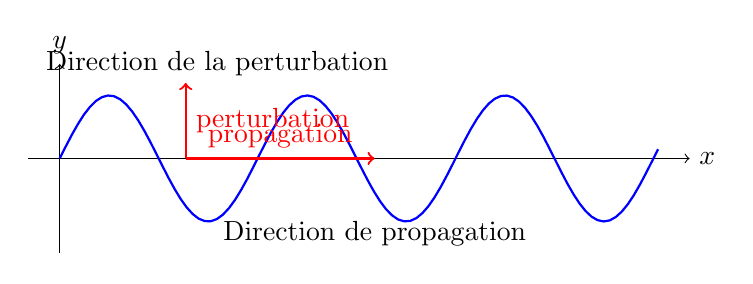
\begin{tikzpicture}[scale=0.8]
% Onde transversale sur une corde
\draw[->] (-0.5,0) -- (10,0) node[right] {$x$};
\draw[->] (0,-1.5) -- (0,1.5) node[above] {$y$};
\draw[thick,blue] plot[domain=0:9.5,samples=100] (\x,{sin(deg(\x*2))});
\draw[thick,red,->] (2,0) -- (2,1.2) node[midway,right] {perturbation};
\draw[thick,red,->] (2,0) -- (5,0) node[midway,above] {propagation};
\node at (5,-1.2) {Direction de propagation};
\node at (2.5,1.5) {Direction de la perturbation};
\end{tikzpicture}
\fig{Figure 8.1 — Onde transversale le long d'une corde. La perturbation est perpendiculaire à la direction de propagation.}
\end{illus}

\subsection{Onde longitudinale}

\begin{definition}[Onde longitudinale]
Une onde est dite \textbf{longitudinale} lorsque la direction de la perturbation est \textbf{parallèle} à la direction de propagation de l'onde.
\end{definition}

\begin{exemple}
Onde le long d'un ressort : on comprime et on relâche une extrémité, les zones de compression et de dilatation se propagent le long du ressort.
\end{exemple}

\begin{illus}
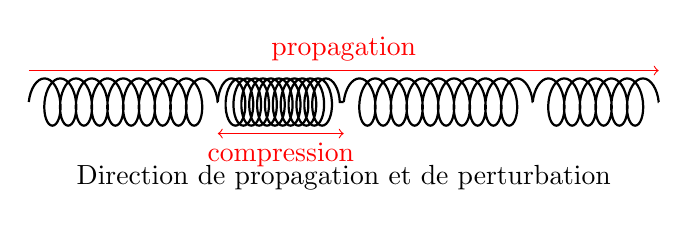
\begin{tikzpicture}[scale=0.8]
% Ressort avec zones de compression
\draw[thick,decorate,decoration={coil,amplitude=3mm,segment length=2mm}] (0,0) -- (3,0);
\draw[thick,decorate,decoration={coil,amplitude=3mm,segment length=1mm}] (3,0) -- (5,0);
\draw[thick,decorate,decoration={coil,amplitude=3mm,segment length=2mm}] (5,0) -- (8,0);
\draw[thick,decorate,decoration={coil,amplitude=3mm,segment length=2mm}] (8,0) -- (10,0);
\draw[red,<->] (3,-0.5) -- (5,-0.5) node[midway,below] {compression};
\draw[red,->] (0,0.5) -- (10,0.5) node[midway,above] {propagation};
\node at (5,-1.2) {Direction de propagation et de perturbation};
\end{tikzpicture}
\fig{Figure 8.2 — Onde longitudinale dans un ressort. Les zones de compression se propagent parallèlement à l'axe.}
\end{illus}

\section{Célérité d'une onde}

\begin{definition}[Célérité]
La \textbf{célérité} (ou vitesse de propagation) d'une onde est la distance parcourue par le front d'onde par unité de temps :
\[
v = \frac{d}{\Delta t}
\]
où $d$ est la distance parcourue pendant la durée $\Delta t$.
\end{definition}

\begin{propriete}[Facteurs influençant la célérité]
La célérité d'une onde mécanique dépend uniquement des propriétés du milieu de propagation (masse volumique, élasticité, température, etc.) et non de la perturbation elle-même.
\end{propriete}

\begin{exemple}
\begin{itemize}
    \item Corde tendue : $v = \sqrt{\frac{T}{\mu}}$ où $T$ est la tension et $\mu$ la masse linéique.
    \item Son dans l'air à \SI{20}{\celsius} : $v \approx \SI{340}{\metre\per\second}$.
    \item Surface de l'eau en eau profonde : $v = \sqrt{\frac{g\lambda}{2\pi}}$.
\end{itemize}
\end{exemple}

\section{Double périodicité des ondes}

\subsection{Périodicité temporelle}

\begin{definition}[Période temporelle]
La \textbf{période temporelle} $T$ est la durée au bout de laquelle un point du milieu retrouve le même état vibratoire. Elle s'exprime en secondes (\si{\second}).
\end{definition}

La fréquence $f$ est l'inverse de la période :
\[
f = \frac{1}{T}
\]
avec $f$ en hertz (\si{\hertz}).

\subsection{Périodicité spatiale}

\begin{definition}[Longueur d'onde]
La \textbf{longueur d'onde} $\lambda$ est la distance séparant deux points consécutifs du milieu qui vibrent en phase. Elle s'exprime en mètres (\si{\metre}).
\end{definition}

\begin{loi}[Relation fondamentale]
Pour une onde progressive sinusoïdale, la célérité $v$, la période $T$ (ou la fréquence $f$) et la longueur d'onde $\lambda$ sont liées par :
\[
\boxed{\lambda = v T = \frac{v}{f}}
\]
\end{loi}

\begin{illus}
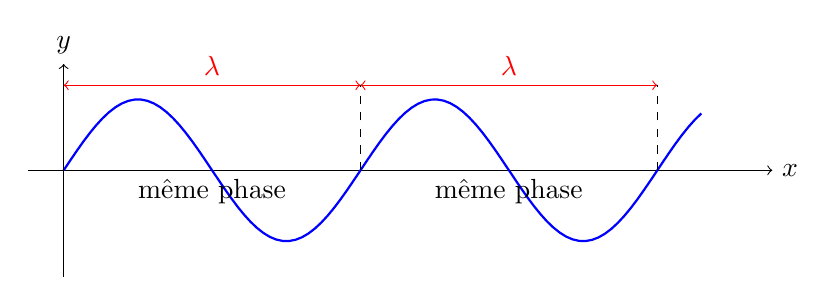
\begin{tikzpicture}[scale=0.9]
\draw[->] (-0.5,0) -- (10,0) node[right] {$x$};
\draw[->] (0,-1.5) -- (0,1.5) node[above] {$y$};
\draw[thick,blue] plot[domain=0:9,samples=100] (\x,{sin(deg(\x*1.5))});
\draw[<->,red] (0,1.2) -- (4.188,1.2) node[midway,above] {$\lambda$};
\draw[<->,red] (4.188,1.2) -- (8.376,1.2) node[midway,above] {$\lambda$};
\draw[dashed] (0,0) -- (0,1.2);
\draw[dashed] (4.188,0) -- (4.188,1.2);
\draw[dashed] (8.376,0) -- (8.376,1.2);
\node at (2.094,-0.3) {même phase};
\node at (6.282,-0.3) {même phase};
\end{tikzpicture}
\fig{Figure 8.3 — Représentation spatiale d'une onde sinusoïdale. La longueur d'onde $\lambda$ est la distance entre deux points en phase.}
\end{illus}

\begin{aretenir}
La double périodicité d'une onde signifie qu'elle est périodique à la fois dans le temps (période $T$) et dans l'espace (longueur d'onde $\lambda$). Ces deux grandeurs sont reliées par $\lambda = vT$.
\end{aretenir}

\section{Ondes à la surface de l'eau}

\subsection{Cuve à ondes}

La cuve à ondes est un dispositif expérimental qui permet d'observer la propagation d'ondes mécaniques à la surface de l'eau. Une lame vibrante crée des perturbations qui se propagent sous forme de rides circulaires.

\begin{experience}[Observation des ondes à la surface de l'eau]
\begin{itemize}
    \item Une lame vibrante plane produit des ondes planes.
    \item Une pointe vibrante produit des ondes circulaires.
    \item En éclairant la cuve avec une lumière stroboscopique, on peut "figer" l'onde et mesurer la longueur d'onde.
\end{itemize}
\end{experience}

\imgreal{ch08-cuve-ondes.png}{Figure — Cuve à ondes : bac d'eau, lame vibrante motorisée, éclairage stroboscopique.}

\subsection{Mesure de la célérité}

Pour mesurer la célérité d'une onde à la surface de l'eau, on peut :
\begin{itemize}
    \item Mesurer la distance $d$ parcourue par le front d'onde pendant une durée $\Delta t$ : $v = d/\Delta t$.
    \item Mesurer la longueur d'onde $\lambda$ et la fréquence $f$ : $v = \lambda f$.
\end{itemize}

\section{Réflexion et réfraction des ondes}

\subsection{Réflexion}

\begin{definition}[Réflexion]
La \textbf{réflexion} est le changement de direction d'une onde lorsqu'elle rencontre une surface séparant deux milieux différents, avec retour dans le milieu initial.
\end{definition}

\begin{loi}[Lois de la réflexion]
\begin{enumerate}
    \item Le rayon incident, le rayon réfléchi et la normale à la surface sont dans le même plan.
    \item L'angle d'incidence $i$ est égal à l'angle de réflexion $r$ : $\boxed{i = r}$.
\end{enumerate}
\end{loi}

\subsection{Réfraction}

\begin{definition}[Réfraction]
La \textbf{réfraction} est le changement de direction d'une onde lorsqu'elle passe d'un milieu à un autre, avec changement de célérité.
\end{definition}

\begin{loi}[Lois de la réfraction (Snell-Descartes)]
\begin{enumerate}
    \item Le rayon incident, le rayon réfracté et la normale sont dans le même plan.
    \item Les angles d'incidence $i_1$ et de réfraction $i_2$ vérifient :
    \[
    \boxed{\frac{\sin i_1}{\sin i_2} = \frac{v_1}{v_2}}
    \]
    où $v_1$ et $v_2$ sont les célérités dans les milieux 1 et 2.
\end{enumerate}
\end{loi}

\begin{illus}
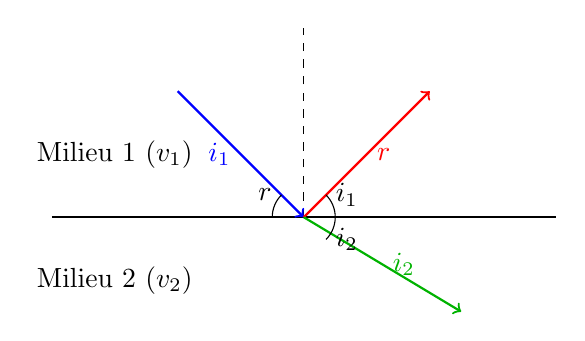
\begin{tikzpicture}[scale=0.8]
% Réflexion et réfraction
\draw[thick] (-4,0) -- (4,0);
\draw[dashed] (0,0) -- (0,3);
\draw[thick,blue,->] (-2,2) -- (0,0) node[midway,left] {$i_1$};
\draw[thick,red,->] (0,0) -- (2,2) node[midway,right] {$r$};
\draw[thick,green!70!black,->] (0,0) -- (2.5,-1.5) node[midway,right] {$i_2$};
\draw (0.5,0) arc (0:45:0.5) node[right] {$i_1$};
\draw (0.5,0) arc (0:-45:0.5) node[right] {$i_2$};
\draw (-0.5,0) arc (180:135:0.5) node[left] {$r$};
\node at (-3,1) {Milieu 1 ($v_1$)};
\node at (-3,-1) {Milieu 2 ($v_2$)};
\end{tikzpicture}
\fig{Figure 8.4 — Réflexion et réfraction d'une onde à l'interface entre deux milieux.}
\end{illus}

\section{Diffraction des ondes}

\begin{definition}[Diffraction]
La \textbf{diffraction} est le phénomène par lequel une onde contourne un obstacle ou s'étale après avoir traversé une ouverture dont les dimensions sont de l'ordre de la longueur d'onde.
\end{definition}

\begin{propriete}[Condition de diffraction]
La diffraction est d'autant plus marquée que la taille de l'obstacle ou de l'ouverture $a$ est petite devant la longueur d'onde $\lambda$ :
\[
a \lesssim \lambda
\]
\end{propriete}

\begin{illus}
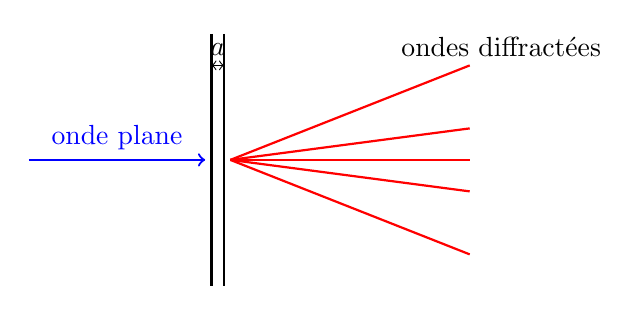
\begin{tikzpicture}[scale=0.8]
% Diffraction par une fente
\draw[thick] (-0.1,2) -- (-0.1,-2);
\draw[thick] (0.1,2) -- (0.1,-2);
\draw[thick,blue,->] (-3,0) -- (-0.2,0) node[midway,above] {onde plane};
\draw[thick,red] (0.2,0) -- (4,1.5);
\draw[thick,red] (0.2,0) -- (4,0.5);
\draw[thick,red] (0.2,0) -- (4,0);
\draw[thick,red] (0.2,0) -- (4,-0.5);
\draw[thick,red] (0.2,0) -- (4,-1.5);
\draw[<->] (-0.1,1.5) -- (0.1,1.5) node[midway,above] {$a$};
\node at (4.5,1.8) {ondes diffractées};
\end{tikzpicture}
\fig{Figure 8.5 — Diffraction d'une onde plane par une fente de largeur $a$. L'onde s'étale dans toutes les directions.}
\end{illus}

\begin{remarque}
La diffraction est un phénomène caractéristique de tous les types d'ondes (mécaniques, électromagnétiques, etc.).
\end{remarque}

\section{Interférences mécaniques}

\subsection{Principe de superposition}

\begin{loi}[Principe de superposition]
Lorsque deux ondes se rencontrent en un point du milieu, l'élongation résultante est la somme algébrique des élongations de chaque onde prise séparément.
\end{loi}

\subsection{Interférences à deux sources}

\begin{definition}[Interférences]
On appelle \textbf{interférences} le phénomène résultant de la superposition de deux ondes cohérentes (même fréquence, différence de phase constante).
\end{definition}

\begin{propriete}[Conditions d'interférences]
Soient deux sources $S_1$ et $S_2$ synchrones émettant des ondes de même amplitude et de même fréquence. En un point $M$ situé à des distances $d_1 = S_1M$ et $d_2 = S_2M$ :
\begin{itemize}
    \item \textbf{Interférence constructive} (amplitude maximale) si la différence de marche $\delta = |d_2 - d_1|$ est un multiple entier de la longueur d'onde :
    \[
    \boxed{\delta = k\lambda \quad (k \in \mathbb{Z})}
    \]
    \item \textbf{Interférence destructive} (amplitude nulle) si la différence de marche est un multiple impair de la demi-longueur d'onde :
    \[
    \boxed{\delta = (2k+1)\frac{\lambda}{2} \quad (k \in \mathbb{Z})}
    \]
\end{itemize}
\end{propriete}

\begin{illus}
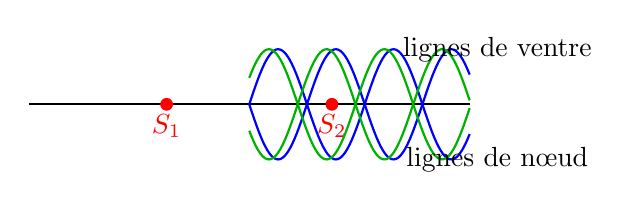
\begin{tikzpicture}[scale=0.7]
% Interférences à deux sources
\draw[thick] (-4,0) -- (4,0);
\filldraw[red] (-1.5,0) circle (3pt) node[below] {$S_1$};
\filldraw[red] (1.5,0) circle (3pt) node[below] {$S_2$};
\draw[blue,thick] plot[domain=0:4,samples=100] (\x,{sin(deg(\x*3))});
\draw[blue,thick] plot[domain=0:4,samples=100] (\x,{-sin(deg(\x*3))});
\draw[green!70!black,thick] plot[domain=0:4,samples=100] (\x,{sin(deg(\x*3+0.5))});
\draw[green!70!black,thick] plot[domain=0:4,samples=100] (\x,{-sin(deg(\x*3+0.5))});
\node at (4.5,1) {lignes de ventre};
\node at (4.5,-1) {lignes de nœud};
\end{tikzpicture}
\fig{Figure 8.6 — Schéma des interférences produites par deux sources ponctuelles synchrones $S_1$ et $S_2$. Les lignes pleines représentent les ventres (interférences constructives), les lignes pointillées les nœuds (interférences destructives).}
\end{illus}

\begin{exemple}
Dans une cuve à ondes, deux pointes vibrantes synchrones produisent des interférences. On observe des zones où l'amplitude est maximale (ventres) et des zones où elle est nulle (nœuds), formant des hyperboles.
\end{exemple}

\begin{aretenir}
Les interférences sont la preuve du caractère ondulatoire de la lumière et des ondes mécaniques. Elles permettent de mesurer précisément la longueur d'onde.
\end{aretenir}

\section{L'essentiel à retenir}

\begin{synthese}
\subsection*{Définitions clés}
\begin{itemize}
    \item \textbf{Onde mécanique} : perturbation se propageant dans un milieu matériel sans transport de matière.
    \item \textbf{Onde transversale} : perturbation $\perp$ direction de propagation.
    \item \textbf{Onde longitudinale} : perturbation $\parallel$ direction de propagation.
    \item \textbf{Célérité} : $v = d/\Delta t$, dépend du milieu.
    \item \textbf{Période temporelle} $T$ : durée d'une vibration complète.
    \item \textbf{Longueur d'onde} $\lambda$ : distance entre deux points en phase.
\end{itemize}

\subsection*{Formules essentielles}
\begin{itemize}
    \item $\boxed{\lambda = vT = \frac{v}{f}}$
    \item Réflexion : $\boxed{i = r}$
    \item Réfraction : $\boxed{\frac{\sin i_1}{\sin i_2} = \frac{v_1}{v_2}}$
    \item Interférences constructives : $\boxed{\delta = k\lambda}$
    \item Interférences destructives : $\boxed{\delta = (2k+1)\frac{\lambda}{2}}$
\end{itemize}

\subsection*{Pièges à éviter}
\begin{itemize}
    \item Ne pas confondre période temporelle $T$ et période spatiale $\lambda$.
    \item La célérité ne dépend pas de la fréquence de l'onde.
    \item La diffraction n'est observable que si $a \lesssim \lambda$.
    \item Pour les interférences, les sources doivent être cohérentes.
\end{itemize}
\end{synthese}

\section{Méthodes \& savoir-faire}

\methode{Calculer la célérité d'une onde}
Pour déterminer la célérité d'une onde :
\begin{enumerate}
    \item Mesurer la distance $d$ parcourue par le front d'onde.
    \item Mesurer la durée $\Delta t$ correspondante.
    \item Appliquer $v = d/\Delta t$.
\end{enumerate}
Ou bien mesurer $\lambda$ et $f$ puis utiliser $v = \lambda f$.

\begin{exemple}
Une onde à la surface de l'eau parcourt \SI{0.5}{\metre} en \SI{2.0}{\second}. Calculer sa célérité.
\medskip

\textbf{Solution :} $v = \frac{d}{\Delta t} = \frac{\SI{0.5}{\metre}}{\SI{2.0}{\second}} = \SI{0.25}{\metre\per\second}$.
\end{exemple}

\methode{Déterminer la longueur d'onde à partir d'une figure d'interférences}
Pour déterminer $\lambda$ à partir d'une figure d'interférences :
\begin{enumerate}
    \item Mesurer la distance entre deux ventres consécutifs (ou deux nœuds consécutifs).
    \item Cette distance est égale à $\lambda/2$ (pour des sources en phase).
    \item En déduire $\lambda$.
\end{enumerate}

\begin{exemple}
Sur une figure d'interférences, la distance entre deux ventres consécutifs est \SI{3.0}{\centi\metre}. La fréquence des sources est \SI{50}{\hertz}. Calculer la célérité de l'onde.
\medskip

\textbf{Solution :} La distance entre deux ventres consécutifs est $\lambda/2$, donc $\lambda = 2 \times \SI{3.0}{\centi\metre} = \SI{6.0}{\centi\metre} = \SI{0.060}{\metre}$. La célérité est $v = \lambda f = \SI{0.060}{\metre} \times \SI{50}{\hertz} = \SI{3.0}{\metre\per\second}$.
\end{exemple}

\methode{Appliquer les lois de la réflexion et de la réfraction}
Pour résoudre un problème de réflexion/réfraction :
\begin{enumerate}
    \item Identifier les milieux et leurs célérités.
    \item Tracer la normale à la surface de séparation.
    \item Mesurer ou calculer l'angle d'incidence.
    \item Appliquer $i = r$ pour la réflexion ou $\frac{\sin i_1}{\sin i_2} = \frac{v_1}{v_2}$ pour la réfraction.
\end{enumerate}

\begin{exemple}
Une onde passe de l'eau ($v_1 = \SI{1500}{\metre\per\second}$) à l'air ($v_2 = \SI{340}{\metre\per\second}$) avec un angle d'incidence de \ang{30}. Calculer l'angle de réfraction.
\medskip

\textbf{Solution :} $\frac{\sin i_1}{\sin i_2} = \frac{v_1}{v_2} \Rightarrow \sin i_2 = \frac{v_2}{v_1} \sin i_1 = \frac{340}{1500} \times \sin\ang{30} = 0.1133$. Donc $i_2 = \arcsin(0.1133) \approx \ang{6.5}$.
\end{exemple}

\methode{Prévoir le type d'interférence en un point}
Pour déterminer si l'interférence est constructive ou destructive en un point $M$ :
\begin{enumerate}
    \item Calculer les distances $d_1 = S_1M$ et $d_2 = S_2M$.
    \item Calculer la différence de marche $\delta = |d_2 - d_1|$.
    \item Comparer $\delta$ à $\lambda$ :
    \begin{itemize}
        \item Si $\delta = k\lambda$ : interférence constructive.
        \item Si $\delta = (2k+1)\lambda/2$ : interférence destructive.
    \end{itemize}
\end{enumerate}

\begin{exemple}
Deux sources synchrones distantes de \SI{4.0}{\centi\metre} émettent des ondes de longueur d'onde $\lambda = \SI{2.0}{\centi\metre}$. Un point $M$ est situé à \SI{5.0}{\centi\metre} de $S_1$ et \SI{7.0}{\centi\metre} de $S_2$. Quel type d'interférence observe-t-on ?
\medskip

\textbf{Solution :} $\delta = |7.0 - 5.0| = \SI{2.0}{\centi\metre} = \lambda$. Donc $\delta = 1 \times \lambda$, interférence constructive.
\end{exemple}

\section{Exercices d'application}

\rubrique{Célérité et longueur d'onde}

\exo{}\diff{1} Une onde progressive sinusoïdale se propage le long d'une corde avec une célérité de \SI{12}{\metre\per\second}. Sa fréquence est \SI{60}{\hertz}. Calculer :
\begin{enumerate}
    \item sa période $T$ ;
    \item sa longueur d'onde $\lambda$.
\end{enumerate}

\exo{}\diff{2} À la surface de l'eau, on mesure une distance de \SI{15}{\centi\metre} entre deux crêtes consécutives. La fréquence de la source est \SI{2.0}{\hertz}. Déterminer la célérité de l'onde.

\exo{}\diff{2} Un vibreur de fréquence \SI{100}{\hertz} produit des ondes à la surface de l'eau. La distance entre le 1\ier{} et le 5\ieme{} front d'onde est \SI{12}{\centi\metre}. Calculer la célérité de l'onde.

\rubrique{Réflexion et réfraction}

\exo{}\diff{1} Une onde sonore se propage dans l'air à \SI{340}{\metre\per\second} et rencontre une paroi. L'angle d'incidence est \ang{45}. Quel est l'angle de réflexion ?

\exo{}\diff{2} Une onde passe de l'eau ($v_1 = \SI{1500}{\metre\per\second}$) à un milieu inconnu avec un angle d'incidence de \ang{40} et un angle de réfraction de \ang{25}. Calculer la célérité dans le second milieu.

\rubrique{Diffraction}

\exo{}\diff{2} Une onde plane de longueur d'onde $\lambda = \SI{3.0}{\centi\metre}$ rencontre une fente de largeur $a = \SI{1.5}{\centi\metre}$. La diffraction est-elle observable ? Justifier.

\exo{}\diff{3} Une onde ultrasonore de fréquence \SI{40}{\kilo\hertz} se propage dans l'air à \SI{340}{\metre\per\second}. Quelle doit être la largeur maximale d'une fente pour observer une diffraction notable ?

\rubrique{Interférences}

\exo{}\diff{2} Deux sources synchrones $S_1$ et $S_2$ distantes de \SI{6.0}{\centi\metre} émettent des ondes de longueur d'onde $\lambda = \SI{2.0}{\centi\metre}$. Un point $M$ est situé à \SI{8.0}{\centi\metre} de $S_1$ et \SI{11.0}{\centi\metre} de $S_2$. 
\begin{enumerate}
    \item Calculer la différence de marche $\delta$.
    \item L'interférence est-elle constructive ou destructive ?
\end{enumerate}

\exo{}\diff{3} Dans une expérience d'interférences à la surface de l'eau, la distance entre deux nœuds consécutifs est \SI{4.0}{\centi\metre}. La fréquence des sources est \SI{5.0}{\hertz}. Calculer la célérité de l'onde.

\section{Exercices d'entraînement}

\rubrique{Célérité et longueur d'onde}

\exo{}\diff{1} Une onde se propage à \SI{20}{\metre\per\second} avec une fréquence de \SI{50}{\hertz}. Quelle est sa longueur d'onde ?

\exo{}\diff{2} La période d'une onde est \SI{0.02}{\second} et sa célérité est \SI{340}{\metre\per\second}. Calculer sa longueur d'onde.

\exo{}\diff{2} Une onde progressive a une longueur d'onde de \SI{5.0}{\centi\metre} et une célérité de \SI{2.0}{\metre\per\second}. Quelle est sa fréquence ?

\exo{}\diff{3} Un vibreur de fréquence réglable produit des ondes à la surface de l'eau. Pour $f = \SI{10}{\hertz}$, la distance entre deux crêtes est \SI{2.5}{\centi\metre}. Pour $f = \SI{20}{\hertz}$, cette distance devient \SI{1.25}{\centi\metre}. Que peut-on conclure sur la célérité ?

\rubrique{Réflexion et réfraction}

\exo{}\diff{1} Une onde lumineuse passe de l'air ($v = \SI{3e8}{\metre\per\second}$) à l'eau ($v = \SI{2.25e8}{\metre\per\second}$) avec un angle d'incidence de \ang{30}. Calculer l'angle de réfraction.

\exo{}\diff{2} Une onde sismique passe d'une couche rocheuse ($v_1 = \SI{5000}{\metre\per\second}$) à une couche sédimentaire ($v_2 = \SI{2000}{\metre\per\second}$). L'angle d'incidence est \ang{60}. L'onde peut-elle se réfracter ? Justifier.

\exo{}\diff{3} Dans une cuve à ondes, une onde plane rencontre un obstacle incliné à \ang{30} par rapport à la direction de propagation. Tracer qualitativement l'onde réfléchie.

\rubrique{Diffraction}

\exo{}\diff{2} Une onde de longueur d'onde $\lambda = \SI{2.0}{\centi\metre}$ rencontre une fente de largeur $a = \SI{0.5}{\centi\metre}$. La diffraction est-elle observable ? Justifier.

\exo{}\diff{3} Pour observer la diffraction d'une onde ultrasonore de fréquence \SI{25}{\kilo\hertz} dans l'air ($v = \SI{340}{\metre\per\second}$), quelle doit être la largeur maximale de la fente ?

\exo{}\diff{3} On réalise la diffraction d'une onde lumineuse de longueur d'onde $\lambda = \SI{500}{\nano\metre}$ par une fente de largeur $a = \SI{0.1}{\milli\metre}$. La diffraction est-elle observable ? Commenter.

\rubrique{Interférences}

\exo{}\diff{2} Deux sources synchrones $S_1$ et $S_2$ distantes de \SI{8.0}{\centi\metre} émettent des ondes de longueur d'onde $\lambda = \SI{3.0}{\centi\metre}$. Un point $M$ est situé à \SI{10.0}{\centi\metre} de $S_1$ et \SI{14.5}{\centi\metre} de $S_2$. 
\begin{enumerate}
    \item Calculer la différence de marche $\delta$.
    \item L'interférence est-elle constructive ou destructive ?
\end{enumerate}

\exo{}\diff{3} Dans une expérience d'interférences, la distance entre le 2\ieme{} et le 5\ieme{} ventre est \SI{9.0}{\centi\metre}. La fréquence des sources est \SI{8.0}{\hertz}. Calculer la célérité de l'onde.

\exo{}\diff{3} Deux haut-parleurs identiques émettent un son de fréquence \SI{440}{\hertz} en phase. Ils sont distants de \SI{2.0}{\metre}. Un microphone est placé à \SI{3.0}{\metre} du premier et \SI{4.0}{\metre} du second. La célérité du son est \SI{340}{\metre\per\second}. Le son perçu est-il intense ou faible ? Justifier.

\section{Sujets type Baccalauréat}

\sujetbac[Ondes à la surface de l'eau]

Dans une cuve à ondes, une lame vibrante produit des ondes planes à la surface de l'eau. La fréquence de vibration est $f = \SI{20}{\hertz}$. On observe que la distance entre deux crêtes consécutives est $d = \SI{1.5}{\centi\metre}$.

\begin{enumerate}
    \item Définir la longueur d'onde $\lambda$. Quelle est sa valeur ici ?
    \item Calculer la célérité $v$ de l'onde.
    \item On place un obstacle plan incliné dans la cuve. Décrire qualitativement ce qui se produit.
    \item On remplace la lame par deux pointes synchrones distantes de $a = \SI{4.0}{\centi\metre}$. 
    \begin{enumerate}
        \item Quel phénomène observe-t-on ?
        \item Un point $M$ est situé à $d_1 = \SI{6.0}{\centi\metre}$ de la première pointe et $d_2 = \SI{7.5}{\centi\metre}$ de la seconde. L'interférence en $M$ est-elle constructive ou destructive ?
    \end{enumerate}
\end{enumerate}

\sujetbac[Onde le long d'une corde]

Une corde élastique de masse linéique $\mu = \SI{0.020}{\kilo\gram\per\metre}$ est tendue horizontalement avec une tension $T = \SI{50}{\newton}$. On impose à son extrémité gauche un mouvement sinusoïdal de fréquence $f = \SI{40}{\hertz}$ et d'amplitude $A = \SI{2.0}{\centi\metre}$.

\begin{enumerate}
    \item Calculer la célérité $v$ de l'onde le long de la corde sachant que $v = \sqrt{T/\mu}$.
    \item Déterminer la longueur d'onde $\lambda$.
    \item Écrire l'équation de l'onde progressive $y(x,t)$ sachant qu'elle se propage dans le sens des $x$ croissants.
    \item À un instant donné, deux points distants de \SI{25}{\centi\metre} vibrent-ils en phase ? Justifier.
    \item L'extrémité droite de la corde est fixe. Décrire le phénomène qui se produit lorsque l'onde atteint cette extrémité.
\end{enumerate}

\section{Corrigés}

\corrige{de l'exercice 1}
\begin{enumerate}
    \item $T = \frac{1}{f} = \frac{1}{60} = \SI{0.0167}{\second}$.
    \item $\lambda = vT = 12 \times 0.0167 = \SI{0.200}{\metre} = \SI{20}{\centi\metre}$.
\end{enumerate}

\corrige{de l'exercice 2}
La distance entre deux crêtes consécutives est la longueur d'onde : $\lambda = \SI{15}{\centi\metre} = \SI{0.15}{\metre}$.
$v = \lambda f = 0.15 \times 2.0 = \SI{0.30}{\metre\per\second}$.

\corrige{de l'exercice 3}
La distance entre le 1\ier{} et le 5\ieme{} front d'onde correspond à $4\lambda$ (car il y a 4 intervalles entre 5 fronts). Donc $4\lambda = \SI{12}{\centi\metre} \Rightarrow \lambda = \SI{3.0}{\centi\metre} = \SI{0.030}{\metre}$.
$v = \lambda f = 0.030 \times 100 = \SI{3.0}{\metre\per\second}$.

\corrige{de l'exercice 4}
D'après la loi de la réflexion, l'angle de réflexion est égal à l'angle d'incidence : $r = i = \ang{45}$.

\corrige{de l'exercice 5}
$\frac{\sin i_1}{\sin i_2} = \frac{v_1}{v_2} \Rightarrow v_2 = v_1 \frac{\sin i_2}{\sin i_1} = 1500 \times \frac{\sin\ang{25}}{\sin\ang{40}} = 1500 \times \frac{0.4226}{0.6428} \approx \SI{986}{\metre\per\second}$.

\corrige{de l'exercice 6}
La diffraction est observable si $a \lesssim \lambda$. Ici $a = \SI{1.5}{\centi\metre}$ et $\lambda = \SI{3.0}{\centi\metre}$, donc $a < \lambda$, la diffraction est observable.

\corrige{de l'exercice 7}
$\lambda = \frac{v}{f} = \frac{340}{40\times 10^3} = \SI{0.0085}{\metre} = \SI{8.5}{\milli\metre}$.
Pour observer une diffraction notable, il faut $a \lesssim \lambda$, donc $a_{\max} \approx \SI{8.5}{\milli\metre}$.

\corrige{de l'exercice 8}
\begin{enumerate}
    \item $\delta = |d_2 - d_1| = |11.0 - 8.0| = \SI{3.0}{\centi\metre}$.
    \item $\lambda = \SI{2.0}{\centi\metre}$, donc $\delta = 1.5\lambda = (2 \times 1 + 1)\lambda/2$. L'interférence est destructive.
\end{enumerate}

\corrige{de l'exercice 9}
La distance entre deux nœuds consécutifs est $\lambda/2$. Donc $\lambda/2 = \SI{4.0}{\centi\metre} \Rightarrow \lambda = \SI{8.0}{\centi\metre} = \SI{0.080}{\metre}$.
$v = \lambda f = 0.080 \times 5.0 = \SI{0.40}{\metre\per\second}$.

\corrige{du sujet 1}
\begin{enumerate}
    \item La longueur d'onde $\lambda$ est la distance entre deux points consécutifs en phase. Ici $\lambda = d = \SI{1.5}{\centi\metre} = \SI{0.015}{\metre}$.
    \item $v = \lambda f = 0.015 \times 20 = \SI{0.30}{\metre\per\second}$.
    \item L'onde subit une réflexion sur l'obstacle incliné. L'angle de réflexion est égal à l'angle d'incidence.
    \item 
    \begin{enumerate}
        \item On observe des interférences : des zones d'amplitude maximale (ventres) et des zones d'amplitude nulle (nœuds).
        \item $\delta = |d_2 - d_1| = |7.5 - 6.0| = \SI{1.5}{\centi\metre} = \lambda$. Donc $\delta = 1 \times \lambda$, interférence constructive.
    \end{enumerate}
\end{enumerate}

\corrige{du sujet 2}
\begin{enumerate}
    \item $v = \sqrt{\frac{T}{\mu}} = \sqrt{\frac{50}{0.020}} = \sqrt{2500} = \SI{50}{\metre\per\second}$.
    \item $\lambda = \frac{v}{f} = \frac{50}{40} = \SI{1.25}{\metre}$.
    \item $y(x,t) = A \sin\left(2\pi ft - \frac{2\pi x}{\lambda}\right) = 0.020 \sin\left(80\pi t - \frac{2\pi x}{1.25}\right)$ (en mètres).
    \item Deux points distants de $\Delta x = \SI{0.25}{\metre}$ vibrent en phase si $\Delta x = k\lambda$. $\frac{\Delta x}{\lambda} = \frac{0.25}{1.25} = 0.2$, ce n'est pas un entier, donc ils ne vibrent pas en phase.
    \item L'onde se réfléchit à l'extrémité fixe. L'onde réfléchie est inversée (changement de signe de l'amplitude) et se superpose à l'onde incidente, créant une onde stationnaire.
\end{enumerate}